\tikzset{every picture/.style={line width=0.75pt}} %set default line width to 0.75pt        

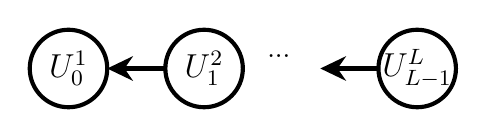
\begin{tikzpicture}[x=0.7pt,y=0.7pt,yscale=-1,xscale=1]
%uncomment if require: \path (0,300); %set diagram left start at 0, and has height of 300

%Shape: Circle [id:dp821654118938725] 
\draw  [line width=1.5]  (40,90) .. controls (40,78.95) and (48.95,70) .. (60,70) .. controls (71.05,70) and (80,78.95) .. (80,90) .. controls (80,101.05) and (71.05,110) .. (60,110) .. controls (48.95,110) and (40,101.05) .. (40,90) -- cycle ;
%Shape: Circle [id:dp9693294242254202] 
\draw  [line width=1.5]  (110,90) .. controls (110,78.95) and (118.95,70) .. (130,70) .. controls (141.05,70) and (150,78.95) .. (150,90) .. controls (150,101.05) and (141.05,110) .. (130,110) .. controls (118.95,110) and (110,101.05) .. (110,90) -- cycle ;
%Straight Lines [id:da7555295343349109] 
\draw [line width=1.5]    (110,90) -- (84,90) ;
\draw [shift={(80,90)}, rotate = 360] [fill={rgb, 255:red, 0; green, 0; blue, 0 }  ][line width=0.08]  [draw opacity=0] (13.4,-6.43) -- (0,0) -- (13.4,6.44) -- (8.9,0) -- cycle    ;
%Straight Lines [id:da1673080699648295] 
\draw [line width=1.5]    (220,90) -- (194,90) ;
\draw [shift={(190,90)}, rotate = 360] [fill={rgb, 255:red, 0; green, 0; blue, 0 }  ][line width=0.08]  [draw opacity=0] (13.4,-6.43) -- (0,0) -- (13.4,6.44) -- (8.9,0) -- cycle    ;
%Shape: Circle [id:dp9339346589837028] 
\draw  [line width=1.5]  (220,90) .. controls (220,78.95) and (228.95,70) .. (240,70) .. controls (251.05,70) and (260,78.95) .. (260,90) .. controls (260,101.05) and (251.05,110) .. (240,110) .. controls (228.95,110) and (220,101.05) .. (220,90) -- cycle ;

% Text Node
\draw (60,90) node  [font=\large]  {$U_{0}^{1}$};
% Text Node
\draw (130,90) node  [font=\large]  {$U_{1}^{2}$};
% Text Node
\draw (161,81) node [anchor=north west][inner sep=0.75pt]   [align=left] {...};
% Text Node
\draw (240,90) node  [font=\large]  {$U_{L-1}^{L}$};


\end{tikzpicture}

